\section{Aplikacja}

\subsection{Wykorzystane technologie}

Aplikacja została zaimplementowana jako aplikacja desktopowa wykorzystująca następujące technologie:
\begin{itemize}
    \item Python jako główny język programowania
    \item PyQt5 do tworzenia interfejsu graficznego
    \item PySwip do integracji z silnikiem Prolog
    \item SWI-Prolog jako silnik wnioskowania
\end{itemize}

\subsection{Architektura systemu}

System składa się z następujących komponentów:
\begin{itemize}
    \item Interfejs użytkownika (GUI) — aplikacja PyQt5
    \item Moduł komunikacji z Prologiem — wykorzystujący bibliotekę PySwip
    \item Baza wiedzy — pliki Prolog zawierające reguły i fakty
    \item Baza danych ofert — pliki CSV z informacjami o nieruchomościach
\end{itemize}

\noindent
Komunikacja między komponentami odbywa się w następujący sposób:
\begin{enumerate}
    \item Użytkownik wchodzi w interakcję z interfejsem GUI
    \item Odpowiedzi użytkownika są konwertowane na format zrozumiały dla Prologa
    \item Zapytania są przekazywane do silnika Prolog poprzez PySwip
    \item Wyniki są przetwarzane i prezentowane użytkownikowi w interfejsie
\end{enumerate}

\subsection{Instrukcja uruchamiania}

Aby uruchomić aplikację:
\begin{enumerate}
    \item Zainstalować wymagane zależności:
    \begin{verbatim}
    pip install -r requirements.txt
    \end{verbatim}
    \item Uruchomić aplikację komendą:
    \begin{verbatim}
    python main.py
    \end{verbatim}
\end{enumerate}

\subsection{Interfejs użytkownika}

Interfejs aplikacji został zaprojektowany w formie okna czatu, które zawiera:
\begin{itemize}
    \item Główny obszar czatu z przewijaniem, wyświetlający historię pytań i odpowiedzi
    \item Dwa przyciski odpowiedzi na dole okna
    \item Ciemny motyw kolorystyczny
    \item Wyraźne formatowanie wiadomości — pytania systemu na jasnym tle, odpowiedzi użytkownika na niebieskim tle
\end{itemize}

\noindent
Rysunki~\ref{fig:preview-1} i~\ref{fig:preview-2} przedstawiają przykładowe uruchomienie aplikacji.
Na pierwszym z nich widoczny jest początek rozmowy i pytanie o wybór rodzaju oferty, zaś drugi obrazuje przykładowe pytania o preferencje.

\begin{figure}[H]
    \centering
    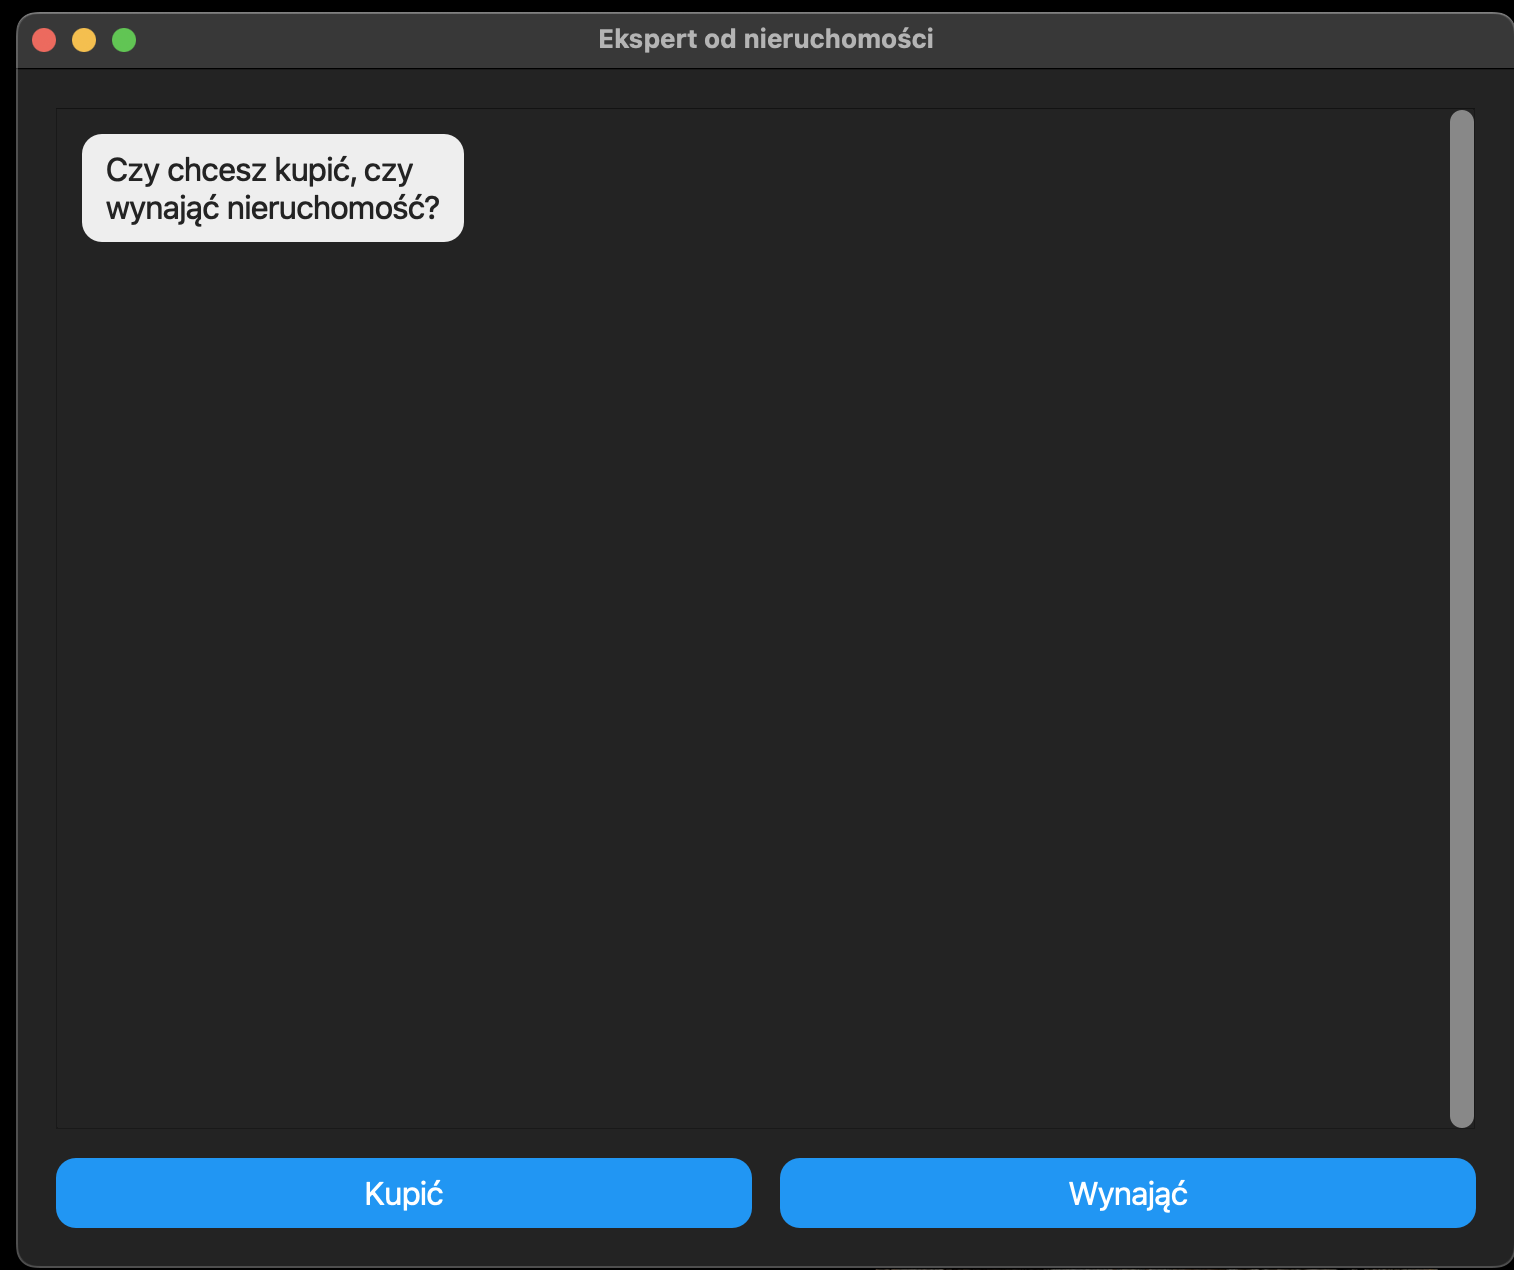
\includegraphics[width=0.9\textwidth]{images/preview-1.png}
    \caption{Interfejs użytkownika: początek rozmowy.}
    \label{fig:preview-1}
\end{figure}

\begin{figure}[H]
    \centering
    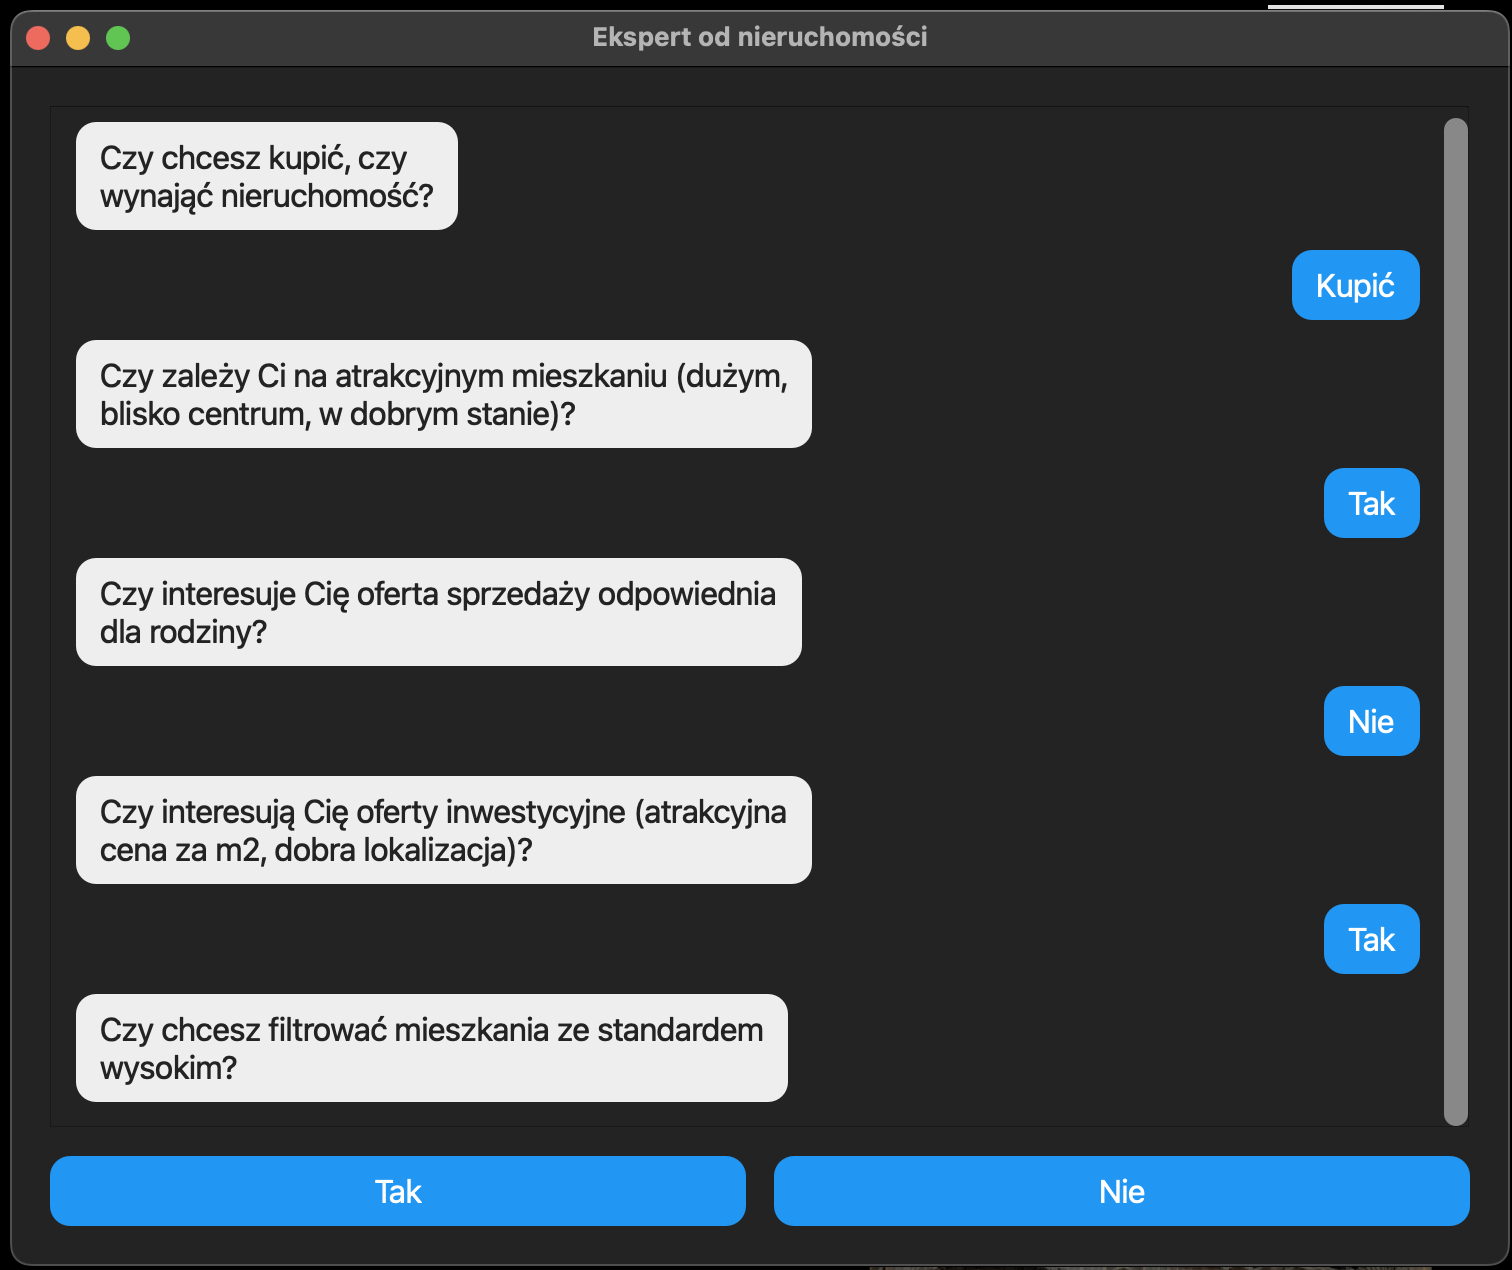
\includegraphics[width=0.9\textwidth]{images/preview-2.png}
    \caption{Interfejs użytkownika: przykładowe pytania o preferencje.}
    \label{fig:preview-2}
\end{figure}

\subsection{Przebieg rozmowy}

Aplikacja prowadzi użytkownika przez proces wyboru nieruchomości w następujący sposób:

\begin{enumerate}
    \item Pierwsze pytanie dotyczy wyboru między kupnem a wynajmem nieruchomości
    \item W zależności od wybranej opcji, system zadaje odpowiedni zestaw pytań o preferencje użytkownika
    \item Każde pytanie wymaga odpowiedzi ``Tak'' albo ``Nie''
    \item Aplikacja wyświetla wynik w postaci listy ofert nieruchomości, które pasują do preferencji użytkownika
\end{enumerate}
W przypadku braku pasujących ofert, system informuje o tym użytkownika odpowiednim komunikatem.
